\documentclass[11pt,letterpaper, twocolumn]{article}
\setlength{\marginparwidth}{2cm}
\usepackage[english]{babel}
\usepackage[utf8x]{inputenc}
\usepackage{amsmath}
\usepackage{amssymb}
\usepackage{graphicx}
\usepackage{tikz}
\usepackage{esvect}
\usepackage[colorinlistoftodos]{todonotes}
\usepackage{enumitem}

\raggedbottom

\author{Etash Jhanji\\\small Collaborators: Josh (TA), Jacob (TA), Colin (TA), \\\small Nathan Banks, Andrew Xia, Rohan Dalal, Akpandu Ekezie}
\title{Physics HW 1}

\begin{document}
\maketitle

\section{1D Collisions}
\begin{enumerate}[label=(\alph*)]
    \item \begin{align*}
        P &= mv\\
        mv_i &= mv_f\\
        v_i &= v_f
    \end{align*}

    \item \begin{center} Frame $p_1$\\ \begin{tikzpicture}
        \draw[thick,->] (0,0) -- (3.4,0) node[anchor=north west] {x axis};
        \draw[thick,->] (0,0) -- (0,3.4) node[anchor=south east] {y axis};
        \draw[thick] (0.5,0) -- (0.5,3.4) node[anchor=north west] {$p_1$};
        \draw[thick, dashed] (2.2,0) -- (0.5,1.7) node[anchor=south east] {};
        \draw[thick, dashed] (0.5,1.7) -- (2.2,3.4) node[anchor=north west] {$p_2$};
    \end{tikzpicture}\end{center} 
    \item \begin{center} Frame $p_2$ \\ \begin{tikzpicture}
        \draw[thick,->] (0,0) -- (3.4,0) node[anchor=north west] {x axis};
        \draw[thick,->] (0,0) -- (0,3.4) node[anchor=south east] {y axis};
        \draw[thick,dashed] (2.2,0) -- (2.2,3.4) node[anchor=north west] {$p_2$};
        \draw[thick] (0.5,0) -- (2.2,1.7) node[anchor=south east] {};
        \draw[thick] (2.2,1.7) -- (0.5,3.4) node[anchor=south west] {$p_1$};
    \end{tikzpicture}\end{center}
    \item \begin{align*}
        \text{Frame } p_1\\
        P_{1s} &= m(0) = 0\\
        P_{2s} &= m(-v) = -mv\\
        E_{1s} &= \frac{1}{2}m(0)^2 = 0\\
        E_{2s} &= \frac{1}{2}m(-v)^2 = \frac{1}{2}mv^2\\
        \text{Frame } p_2\\
        P_{1s} &= m(v) = mv\\
        P_{2s} &= m(0) = 0\\
        E_{1s} &= \frac{1}{2}m(v)^2 = \frac{1}{2}mv^2\\
        E_{2s} &= \frac{1}{2}m(0)^2 = 0\\
    \end{align*}
    \item \begin{align*}
        \text{Frame } p_1\\
        P_{1f} &= m(0) = 0\\
        P_{2f} &= m(v) = mv\\
        E_{1f} &= \frac{1}{2}m(0)^2 = 0\\
        E_{2f} &= \frac{1}{2}m(v)^2 = \frac{1}{2}mv^2\\
        \text{Frame } p_2\\
        P_{1f} &= m(-v) = -mv\\
        P_{2f} &= m(0) = 0\\
        E_{1f} &= \frac{1}{2}m(-v)^2 = \frac{1}{2}mv^2\\
        E_{2f} &= \frac{1}{2}m(0)^2 = 0\\
    \end{align*}
\end{enumerate}

\section{2D Collisions}
\begin{enumerate}[label=(\alph*)]
    \item \begin{center}
    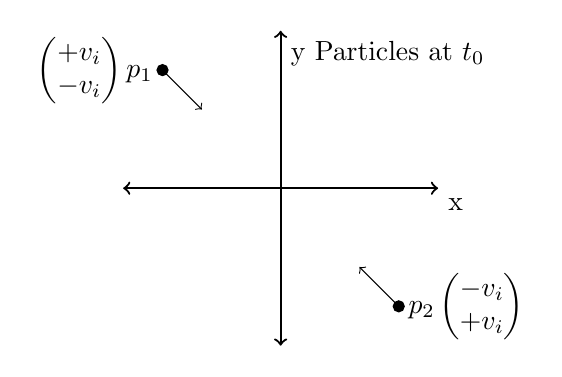
\begin{tikzpicture}
        \draw[thick, <->](0,2) -- (4,2) node[anchor=north west] {x};
        \draw[thick, <->](2,0) -- (2,4) node[anchor=north west] {y  Particles at $t_0$};
        \filldraw[black] (0.5,3.5) circle (2pt) node[anchor=east]{$\begin{pmatrix}+v_i\\-v_i\end{pmatrix} p_1$};
        \filldraw[black] (3.5,0.5) circle (2pt) node[anchor=west]{$p_2 \begin{pmatrix}-v_i\\+v_i\end{pmatrix}$};
        \draw[->](0.5, 3.5) -- (1, 3) node[anchor=north west] {};
        \draw[->](3.5, 0.5) -- (3, 1) node[anchor=north west] {};
    \end{tikzpicture}
\end{center}
    \item \begin{align*}
            E&=mv^2\\
            \sum{E_i} &= 2[\frac{1}{2}m(\|\vv{v_i}\|)]\\
            \sum{E_f} &= 2[\frac{1}{2}m(\|\vv{v_f}\|)]\\
            \sum{E_i} &= \sum{E_f}\\
            \|\vv{v_f}\| &= \|\vv{v_i}\|
        \end{align*}
        \begin{align*}
            \vv{P_{1i}} + \vv{P_{2i}} &= 0 \\
            \therefore \vv{P_{1f}} + \vv{P_{2f}} &= 0 \\
            -\begin{pmatrix}
                +v_f\\+v_f
            \end{pmatrix} &= \vv{P_{2f}}\\
        \vv{P_{2f}} &= \begin{pmatrix}
            -v_f\\-v_f
        \end{pmatrix} 
    \end{align*}
    \item \begin{center}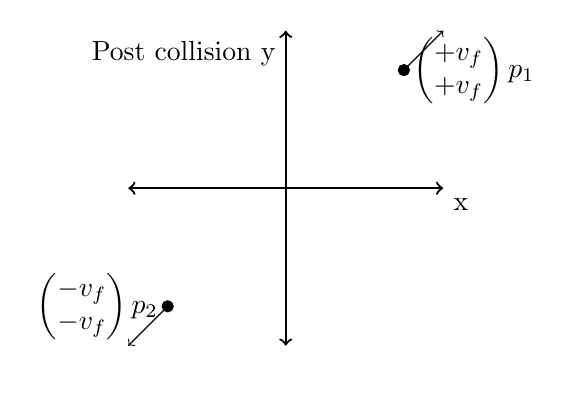
\begin{tikzpicture}
        \draw[thick, <->](0,2) -- (4,2) node[anchor=north west] {x};
        \draw[thick, <->](2,0) -- (2,4) node[anchor=north east] {Post collision y};
        \filldraw[black] (3.5,3.5) circle (2pt) node[anchor=west]{$\begin{pmatrix}+v_f\\+v_f\end{pmatrix} p_1$};
        \filldraw[black] (0.5,0.5) circle (2pt) node[anchor=east]{$\begin{pmatrix}-v_f\\-v_f\end{pmatrix} p_2$};
        \draw[->](3.5, 3.5) -- (4, 4) node[anchor=north west] {};
        \draw[->](0.5, 0.5) -- (0, 0) node[anchor=north west] {};
    \end{tikzpicture}\end{center}
    \item \begin{center}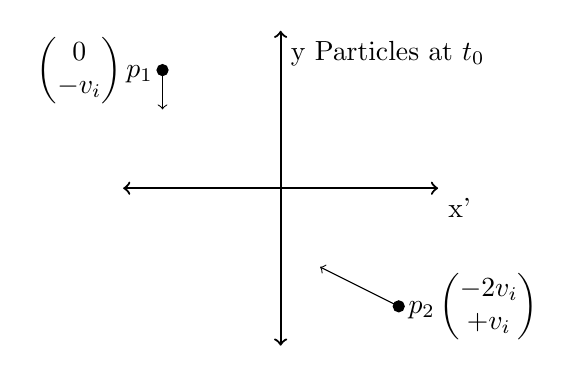
\begin{tikzpicture}
        \draw[thick, <->](0,2) -- (4,2) node[anchor=north west] {x'};
        \draw[thick, <->](2,0) -- (2,4) node[anchor=north west] {y  Particles at $t_0$};
        \filldraw[black] (0.5,3.5) circle (2pt) node[anchor=east]{$\begin{pmatrix}0\\-v_i\end{pmatrix} p_1$};
        \filldraw[black] (3.5,0.5) circle (2pt) node[anchor=west]{$p_2 \begin{pmatrix}-2v_i\\+v_i\end{pmatrix}$};
        \draw[->](0.5, 3.5) -- (0.5, 3) node[anchor=north west] {};
        \draw[->](3.5, 0.5) -- (2.5, 1) node[anchor=north west] {};
    \end{tikzpicture}\end{center}
    \begin{center}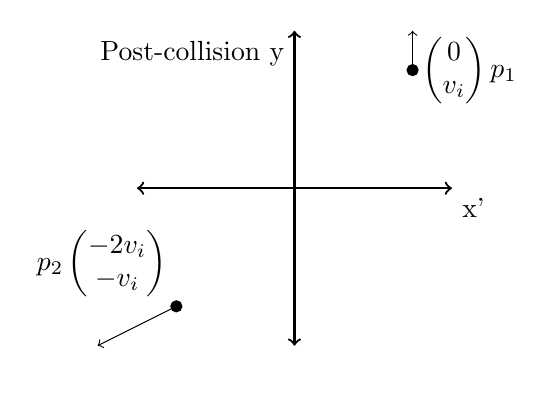
\begin{tikzpicture}
        \draw[thick, <->](0,2) -- (4,2) node[anchor=north west] {x'};
        \draw[thick, <->](2,0) -- (2,4) node[anchor=north east] {Post-collision  y};
        \filldraw[black] (3.5,3.5) circle (2pt) node[anchor=west]{$\begin{pmatrix}0\\v_i\end{pmatrix} p_1$};
        \filldraw[black] (0.5,0.5) circle (2pt) node[anchor=south east]{$p_2 \begin{pmatrix}-2v_i\\-v_i\end{pmatrix}$};
        \draw[->](3.5, 3.5) -- (3.5, 4) node[anchor=north west] {};
        \draw[->](0.5, 0.5) -- (-0.5, 0) node[anchor=north west] {};
    \end{tikzpicture}\end{center}
    \item \begin{align*}
        v_{1ix}'&=v_{1ix}-v_{frame}\\
        v_{1ix}'&=v_{ix}-v_{i}\\
        v_{1ix}'&=0\\
        \vv{v_{1i}}&=\begin{pmatrix}0\\-v_i\end{pmatrix}\\
    \end{align*}
    \begin{align*}
        v_{2ix}'&=-v_{2ix}-v_{frame}\\
        v_{2ix}'&=-v_{ix}-v_{i}\\
        v_{2ix}'&=-2v_{i}\\
        \vv{v_{2i}}&=\begin{pmatrix}-2v_i\\v_i\end{pmatrix}
    \end{align*}
    \begin{align*}
        v_{1fx}'&=v_{1fx}-v_{frame}\\
        v_{1fx}'&=v_{ix}-v_{i}\\
        v_{1fx}'&=0\\
        \vv{v_{1f}}&=\begin{pmatrix}0\\v_i\end{pmatrix}\\
    \end{align*}
    \begin{align*}
        v_{2fx}'&=-v_{2ix}-v_{frame}\\
        v_{2fx}'&=-v_{ix}-v_{i}\\
        v_{2fx}'&=-2v_{i}\\
        \vv{v_{2f}}&=\begin{pmatrix}-2v_i\\-v_i\end{pmatrix}
    \end{align*}
    \item \begin{align*}
        \text{Frame 1}\\
        P_{1xi} &= +mv_i\\
        P_{1yi} &= -mv_i\\
        P_{2xi} &= -mv_i\\
        P_{2yi} &= +mv_i\\
        E_{1i} &= \frac{1}{2}m||\vv{v_i}||^2\\
        E_{1i} &= \frac{1}{2}m(\sqrt{v_{i}^2 + (-v_{i})^2})^2\\
        E_{1i} &= mv_{i}^2\\
        E_{2i} &= \frac{1}{2}m||\vv{v_i}||^2\\
        E_{2i} &= mv_{i}^2\\\\
        P_{1xf} &= +mv_f\\
        P_{1yf} &= +mv_f\\
        P_{2xf} &= -mv_f\\
        P_{2yf} &= -mv_f\\
        E_{1f} &= \frac{1}{2}m||\vv{v_f}||^2\\
        E_{1f} &= \frac{1}{2}m(\sqrt{v_{f}^2 + v_{f}^2})^2\\
        E_{1f} &= mv_{f}^2\\
        E_{2f} &= \frac{1}{2}m||\vv{v_f}||^2\\
        E_{2f} &= mv_{f}^2\\
    \end{align*}
    \begin{align*}
        \text{Moving Frame}\\
        P_{1xi}' &= m(0) = 0\\
        P_{1yi}' &= -mv_i\\
        P_{2xi}' &= -2mv_i\\
        P_{2yi}' &= +mv_i\\
        E_{1i}' &= \frac{1}{2}m||\vv{v_{1i}'}||^2\\
        E_{1i}' &= \frac{1}{2}m(\sqrt{0^2 + (-v_{i})^2})^2\\
        E_{1i}' &= \frac{1}{2}mv_{i}^2\\
        E_{2i}' &= \frac{1}{2}m||\vv{v_i}||^2\\
        E_{1i}' &= \frac{1}{2}m(\sqrt{(-2v_i)^2 + (v_{i})^2})^2\\
        E_{1i}' &= \frac{5}{2}mv_{i}^2\\\\
        P_{1xf}' &= m(0) = 0\\
        P_{1yf}' &= +mv_f\\
        P_{2xf}' &= -2mv_f\\
        P_{2yf}' &= -mv_f\\
        E_{1f}' &= \frac{1}{2}m||\vv{v_f}||^2\\
        E_{1f}' &= \frac{1}{2}m(\sqrt{0^2 + v_{i}^2})^2\\
        E_{1f}' &= \frac{1}{2}mv_{i}^2\\
        E_{2f}' &= \frac{1}{2}m||\vv{v_f}||^2\\
        E_{1f}' &= \frac{1}{2}m(\sqrt{(-2v_{i})^2 + (-v_{i})^2})^2\\
        E_{2f}' &= \frac{5}{2}mv_{i}^2\\
    \end{align*}
\end{enumerate}

\section{Matrix Multiplication}
\begin{enumerate}[label=(\alph*)]
    \item \begin{align*}
            A \times C &= \begin{pmatrix}
                a_{11}c_{1} + a_{12}c_{2}\\a_{21}c_{1} + a_{22}c_{2}
            \end{pmatrix}
        \end{align*}
    \item \begin{align*}
        A \times B &= \begin{pmatrix}
            a_{11}b_{11} + a_{12}b_{21} & a_{11}b_{12} + a_{12}b_{22}\\
            a_{21}b_{11} + a_{22}b_{21} & a_{21}b_{12} + a_{22}b_{22}
        \end{pmatrix}
    \end{align*}
    \item \begin{align*}
        n \times A &= \begin{pmatrix}
            na_{11} & na_{11}\\
            na_{21} & na_{21}
        \end{pmatrix}
    \end{align*}
\end{enumerate}

\section{Proton Collisions in Newtonian Mechanics}

\begin{align*}
    0&=mv_{f1}^2\sin\theta + mv_{f2}^2\sin-\theta\\
    v_{f1}&=v_{f2}\\
\end{align*}
\begin{align*}
    E_i &= \frac{1}{2}mv_i^2\\
    E_{f} &= 2[\frac{1}{2}mv_f^2\\
    E_{f} &= mv_f^2\\
    E_f &= E_i\\
    \frac{1}{2}mv_i^2 &= mv_f^2\\
    v_f &= \frac{v_i}{\sqrt{2}}\\
\end{align*}
\begin{align*}
    P_{xi} &= P_{xf}\\
    mv_i &= 2mv_f\cos\theta\\
    v_i&=2v_f\cos\theta\\
    v_i &= 2m(\frac{v_i}{\sqrt{2}})\cos\theta\\
    \frac{\sqrt{2}v_i}{2v_i} &= \cos\theta\\
    \theta &= \arccos{\frac{\sqrt{2}}{2}}\\
    \theta &= \frac{\pi}{4} = 45\text{\textdegree }
\end{align*}

\section{(Challenge Problem) General Linear Coordinate Transformations}
\begin{enumerate}[label=(\alph*)]
    \item \begin{align*}
        \begin{pmatrix}x\\t\end{pmatrix} &= \begin{pmatrix}a&b\\e&f\end{pmatrix}\begin{pmatrix}x'\\t'\end{pmatrix}\\
        \text{Given }x&=vt\text{ when }x'=0\\
        \begin{pmatrix}vt\\t\end{pmatrix} &= \begin{pmatrix}a&b\\e&f\end{pmatrix}\begin{pmatrix}0\\t'\end{pmatrix}\\
        \begin{pmatrix}vt\\t\end{pmatrix} &= \begin{pmatrix}bt'\\ft'\end{pmatrix}\\
        t&=ft'\\
        vt &= bt'\\
        vft'&=bt'\\
        b&=vf
    \end{align*}
    \item \begin{align*}
        \begin{pmatrix}x\\t\end{pmatrix} &= \begin{pmatrix}a&vf\\e&f\end{pmatrix}\begin{pmatrix}x'\\t'\end{pmatrix}\\
        \text{Given }x'&=vt'\text{ when }x=0\\
        \begin{pmatrix}0\\t\end{pmatrix} &= \begin{pmatrix}a&vf\\e&f\end{pmatrix}\begin{pmatrix}-vt'\\t'\end{pmatrix}\\
        \begin{pmatrix}0\\t\end{pmatrix} &= \begin{pmatrix}-avt'+vft'\\-evt'+ft'\end{pmatrix}\\
        avt'&=vft'\\
        a&=f\\
    \end{align*}
    \item \begin{align*}
        \begin{pmatrix}x\\t\end{pmatrix} &= \begin{pmatrix}f&vf\\e&f\end{pmatrix}\begin{pmatrix}x'\\t'\end{pmatrix}\\
        T(v_1)T(v_2) &= T(v_f)\\
        &=\begin{pmatrix}f_1&v_1f_1\\e_1&f_1\end{pmatrix}\begin{pmatrix}f_2&v_2f_2\\e_2&f_2\end{pmatrix}\\
        &=\begin{pmatrix}f_1f_2+f_1v_1e_2 & f_1v_2f_2+f_1v_1f_2\\e_1f_2+f_1e_2 & e_1v_2f_2+f_1f_2\end{pmatrix}\\
        f_1f_2+f_1v_1e_2 &= e_1v_2f_2+f_1f_2\\
        \frac{f_1v_1}{e_1} &= \frac{f_2v_2}{e_2}\\
        g &= \frac{vf}{e}\\
        e &= \frac{vf}{g}\\
    \end{align*}
    \item \begin{align*}
        \begin{pmatrix}x\\t\end{pmatrix} &= \begin{pmatrix}f&vf\\\frac{vf}{g}&f\end{pmatrix}\begin{pmatrix}x'\\t'\end{pmatrix}\\
        T(v)T(-v) &= T(0)\\
        &=\begin{pmatrix}f&vf\\\frac{vf}{g}&f\end{pmatrix}\begin{pmatrix}f&-vf\\\frac{-vf}{g}&f\end{pmatrix}\\
        &= \begin{pmatrix}f^2-\frac{v^2f^2}{g} & -vf^2+vf^2\\\frac{vf^2}{g}-\frac{vf^2}{g} & f^2-\frac{v^2f^2}{g}\end{pmatrix}\\
        &= \begin{pmatrix}f^2-\frac{v^2f^2}{g} & 0\\0 & f^2-\frac{v^2f^2}{g}\end{pmatrix}\\
        \begin{pmatrix}x\\t\end{pmatrix} &= \begin{pmatrix}f^2-\frac{v^2f^2}{g} & 0\\0 & f^2-\frac{v^2f^2}{g}\end{pmatrix}\begin{pmatrix}x'\\t'\end{pmatrix}\\
        \begin{pmatrix}x\\t\end{pmatrix} &= \begin{pmatrix}x'(f^2-\frac{v^2f^2}{g})\\t'(f^2-\frac{v^2f^2}{g})\end{pmatrix}\\
        x &= x'(f^2-\frac{v^2f^2}{g})\\
        1&=f^2-\frac{v^2f^2}{g}\\
        f&=\frac{1}{\sqrt{1-\frac{v^2}{g}}}
    \end{align*}
    \item\begin{align*}
        \begin{pmatrix}x\\t\end{pmatrix}&= \frac{1}{\sqrt{1-\frac{v^2}{g}}}\begin{pmatrix}1 & v \\ \frac{v}{g} & 1\end{pmatrix}\begin{pmatrix}x'\\t'\end{pmatrix}\\
        g&=v_*^2\\
        \begin{pmatrix}x\\t\end{pmatrix}&= \frac{1}{\sqrt{1-\frac{v^2}{v_*^2}}}\begin{pmatrix}1 & v \\ \frac{v}{v_*^2} & 1\end{pmatrix}\begin{pmatrix}x'\\t'\end{pmatrix}\\
    \end{align*}
    Take $x'=v_*t'$
    \begin{align*}
        \begin{pmatrix}x\\t\end{pmatrix}&= \frac{1}{\sqrt{1-\frac{v_*^2}{v_*^2}}}\begin{pmatrix}1 & v_* \\ -\frac{v_*}{v_*^2} & 1\end{pmatrix}\begin{pmatrix}x'\\t'\end{pmatrix}\\
        t&= \frac{1}{\sqrt{1-\frac{v_*^2}{v_*^2}}}(-\frac{x'v_*}{v_*^2}+t')\\
        t'&=\frac{x'}{v_*}\\
        x'&=v_*t'
    \end{align*} 
    \item \begin{align*}
        v_*&^2t^2-x^2=v_*^2t'^2-x'^2\\
        \begin{pmatrix}x\\t\end{pmatrix}&= \frac{1}{\sqrt{1-\frac{v^2}{v_*^2}}}\begin{pmatrix}1 & v \\ \frac{v}{v_*^2} & 1\end{pmatrix}\begin{pmatrix}x'\\t'\end{pmatrix}\\
        \text{Let }\gamma &= \frac{1}{\sqrt{1-\frac{v^2}{v_*^2}}}\\
        \begin{pmatrix}x\\t\end{pmatrix}&= \gamma\begin{pmatrix}1 & v \\ \frac{v}{v_*^2} & 1\end{pmatrix}\begin{pmatrix}x'\\t'\end{pmatrix}\\
        \begin{pmatrix}x\\t\end{pmatrix}&= \gamma\begin{pmatrix}x'+vt' \\ x'\frac{v}{v_*^2}+t'\end{pmatrix}\\
        x&=\gamma(x'+vt')\\
        t&=\gamma(x'\frac{v}{v_*^2}+t')\\
        v_*^2&[\gamma(x'(\frac{v}{v_*^2})+t')]^2-[\gamma(x'+vt')]^2\\
        &=\gamma^2[[v_*^2(x'(\frac{v}{v_*^2})+t')^2]-(x'+vt')^2]\\
        &= \gamma^2[(\frac{x'^2v^2}{v_*^2}+t'^2v_*^2)-x'^2-v^2t'^2]\\
        &=\frac{1}{1-\frac{v^2}{v_*^2}}[t'^2(v_*^2-v^2)-x'^2(1-\frac{v^2}{v_*^2})]\\
        &=\frac{t'^2(v_*^2-v^2)}{1-\frac{v^2}{v_*^2}}-x'^2\\
        &=v_*^2t'^2-x'^2\\
    \end{align*}
    \item $v_* = \infty$
\end{enumerate}

\section{How long does it take light to travel a foot?}
\begin{align*}
    1\text{ft} &= ct\\
    t &= \frac{1\text{ft}}{c}\\
    c&=3 \cdot 10^8  \text{ from BYJU's}\\
    t &= 0.3048\text{m} \cdot \frac{1\text{s}}{3 \cdot 10^8\text{m}}\\
    t &= 1.016 \cdot 10^{-9} \text{s}
\end{align*}

\section{Two Runners}
\begin{align*}
    \text{Runner B}\\
    t_B &= \frac{L}{v}\\
    \text{Runner A}\\
    t_A &= \frac{\frac{L}{2}}{2v} + \frac{\frac{L}{2}}{\frac{v}{2}}\\
    t_A &= \frac{L}{4v} + \frac{L}{v}\\
    \\
    \frac{L}{4v} + \frac{L}{v} &> \frac{L}{v}\\
    t_A&>t_B\\
    \text{Runner B wins}\\
\end{align*}

\end{document}